\documentclass{article} % For LaTeX2e
\usepackage{nips14submit_e,times}
\usepackage{amsmath}
\usepackage{amsthm}
\usepackage{amssymb}
\usepackage{mathtools}
\usepackage{hyperref}
\usepackage{url}
\usepackage{algorithm}
\usepackage[noend]{algpseudocode}
%\documentstyle[nips14submit_09,times,art10]{article} % For LaTeX 2.09

\usepackage{mathrsfs}
\usepackage{graphicx}
\usepackage{caption}
\usepackage{subcaption}

\def\eQb#1\eQe{\begin{eqnarray*}#1\end{eqnarray*}}
\def\aB#1\aE{\begin{align*}#1\end{align*}}
\def\eQnb#1\eQne{\begin{align}#1\end{align}}
\providecommand{\e}[1]{\ensuremath{\times 10^{#1}}}
\providecommand{\pb}[0]{\pagebreak}

\newcommand{\E}{\mathrm{E}}
\newcommand{\Var}{\mathrm{Var}}
\newcommand{\Cov}{\mathrm{Cov}}

\def\Qb#1\Qe{\begin{question}#1\end{question}}
\def\Sb#1\Se{\begin{solution}#1\end{solution}}

\newenvironment{claim}[1]{\par\noindent\underline{Claim:}\space#1}{}
\newtheoremstyle{quest}{\topsep}{\topsep}{}{}{\bfseries}{}{ }{\thmname{#1}\thmnote{ #3}.}
\theoremstyle{quest}
\newtheorem*{definition}{Definition}
\newtheorem*{theorem}{Theorem}
\newtheorem*{lemma}{Lemma}
\newtheorem*{question}{Question}
\newtheorem*{preposition}{Preposition}
\newtheorem*{exercise}{Exercise}
\newtheorem*{challengeproblem}{Challenge Problem}
\newtheorem*{solution}{Solution}
\newtheorem*{remark}{Remark}
\usepackage{verbatimbox}
\usepackage{listings}
\title{Harmonic Analysis:  \\
Problem Set II}


\author{
Youngduck Choi \\
CIMS \\
New York University\\
\texttt{yc1104@nyu.edu} \\
}


% The \author macro works with any number of authors. There are two commands
% used to separate the names and addresses of multiple authors: \And and \AND.
%
% Using \And between authors leaves it to \LaTeX{} to determine where to break
% the lines. Using \AND forces a linebreak at that point. So, if \LaTeX{}
% puts 3 of 4 authors names on the first line, and the last on the second
% line, try using \AND instead of \And before the third author name.

\newcommand{\fix}{\marginpar{FIX}}
\newcommand{\new}{\marginpar{NEW}}

\nipsfinalcopy % Uncomment for camera-ready version

\begin{document}


\maketitle

\begin{abstract}
This work contains solutions to the problem set II
of Harmonic Analysis 2016 at Courant Institute of Mathematical Sciences.
\end{abstract}

\begin{question}[1]
\hfill
\begin{figure}[h!]
  \centering
    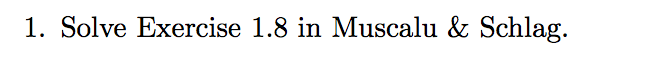
\includegraphics[width=0.5\textwidth]{HA-2-1.png}
\end{figure}
\end{question}

\begin{solution}
\end{solution}

\newpage

\begin{question}[2]
\hfill
\begin{figure}[h!]
  \centering
    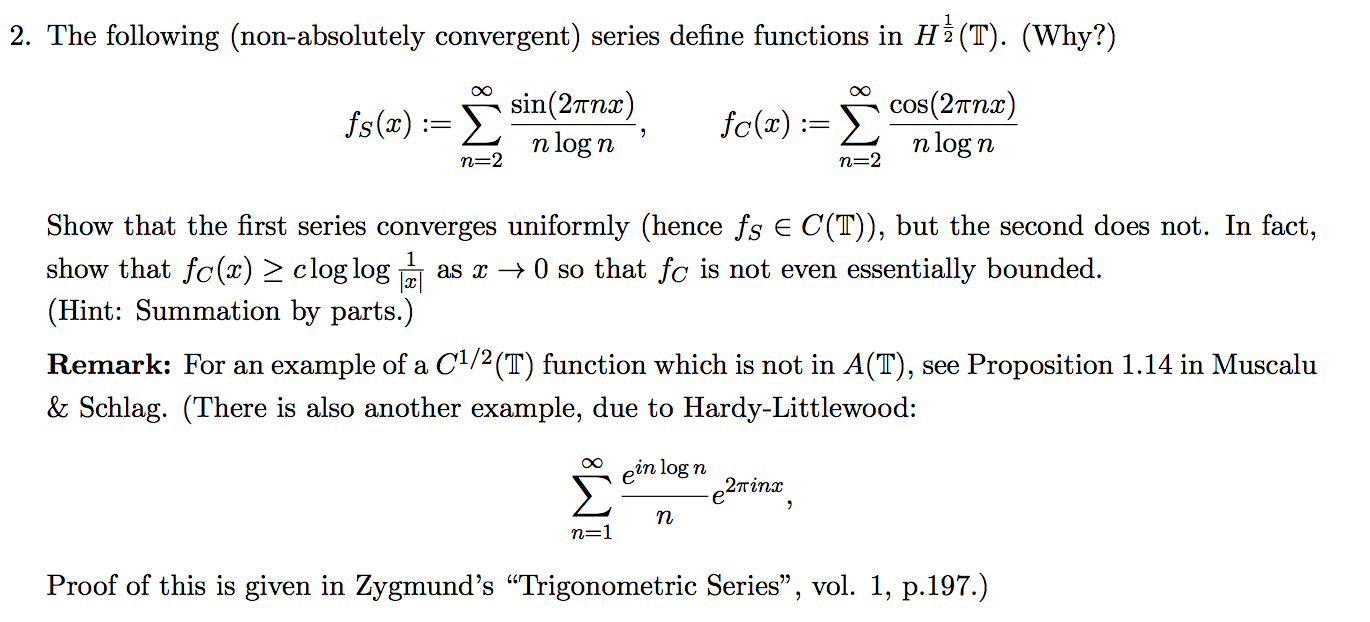
\includegraphics[width=1\textwidth]{HA-2-2.png}
\end{figure}
\end{question}
\begin{solution}
Define $g_{n,m} =
 \sum_{i = n}^{m} \dfrac{\sin(2\pi n x)}{n\log(n)}$. 
For $x \in [0,\dfrac{1}{m}]$, we have
\eQb
|g_{n,m}| &\leq& 
\sum_{i = n}^{m} \left| \dfrac{\sin(2\pi i x)}{i\log(i)} \right| 
\leq \sum_{i=n}^{m} \dfrac{2\pi i x}{i \log(i)} = \sum_{i=n}^{m} \dfrac{2 \pi x}{\log(i)} \\
&\leq& \dfrac{1}{\log(n)}  
\leq \dfrac{1}{m\log(n)} \sum_{i = n}^{m}{2\pi} \leq \dfrac{2\pi}{\log(n)}.  \\
\eQe
For $x \in [\dfrac{1}{m}, \dfrac{1}{n}]$, we obtain 

Therefore, we have that 
\eQb
|g_{n,m}| = O(\dfrac{1}{log(n)}),
\eQe
and the partial sums of $f_S$ is cauchy. Thus, $f_S$ converges uniformly and $f \in C(\mathbb{T})$.

\end{solution}

\newpage

\begin{question}[3]
\hfill
\begin{figure}[h!]
  \centering
    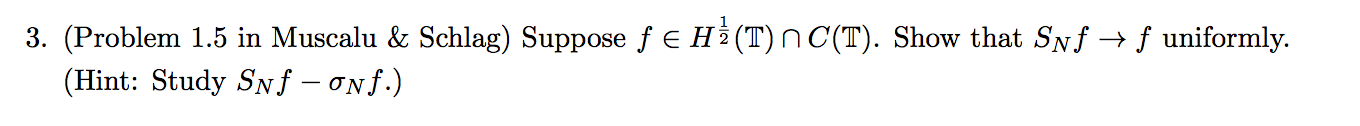
\includegraphics[width=1\textwidth]{HA-2-3.png}
\end{figure}
\end{question}
\begin{solution} 
By the triangle inequality of the supnorm, we have
\eQb
||S_N f - f ||_{\infty} \leq ||S_N f - \sigma_N f ||_{\infty} + 
||\sigma_N f - f||_{\infty},
\eQe
for all $N \in \mathbb{Z}^{+}$. As $f \in C(\mathbb{T})$, we have that 
$||\sigma_N f - f||_{\infty} \to 0$ as $N \to \infty$.
Therefore, by the linearity of limit, 
it suffices to show that $||S_N f - \sigma_N f||_{\infty} \to 0$ as $N \to \infty$. 
By definition of $S_N$ and $\sigma_N$, triangle inequality, and Cauchy-Schwarz, we obtain 
\eQb
||S_N f - \sigma_N f||_{\infty} =  &\leq& \sum_{n = -N}^{N} \dfrac{|n|}{N}|\hat{f}(n)| \\
&\leq& \sum_{n=-M}^{M} \dfrac{|n||\hat{f}(n)|}{N} + (\sum_{N \geq |n| > M} \dfrac{|n|}{N^2})^{\frac{1}{2}}
(\sum_{N \geq |n| > M}|n||\hat{f}(n)|^2)^{\frac{1}{2}}, \\ 
&\leq& \sum_{n=-M}^{M} \dfrac{|n||\hat{f}(n)|}{N} + 
2(\sum_{N \geq |n| > M}|n||\hat{f}(n)|^2)^{\frac{1}{2}}, \\ 
\eQe
for any $N > M$. Taking $\limsup$ with respect to $N$ on both sides, we get
\eQb
\limsup_{N \to \infty} ||S_N f - \sigma_N f||_{\infty} &\leq&
2(\sum_{|n| > M}|n||\hat{f}(n)|^2)^{\frac{1}{2}}, \\ 
\eQe
As $f \in H^{\frac{1}{2}}(\mathbb{T})$, taking the limit as $M \to \infty$ gives
\eQb
\limsup_{N \to \infty} ||S_N f - \sigma_N f||_{\infty} &\leq& 0
\eQe
Hence, we have shown that $||S_N f - \sigma_N f||_{\infty} \to 0$ as $N \to \infty$ as desired. 
\hfill $\qed$
\end{solution}

\newpage

\begin{question}[4]
\hfill
\begin{figure}[h!]
  \centering
    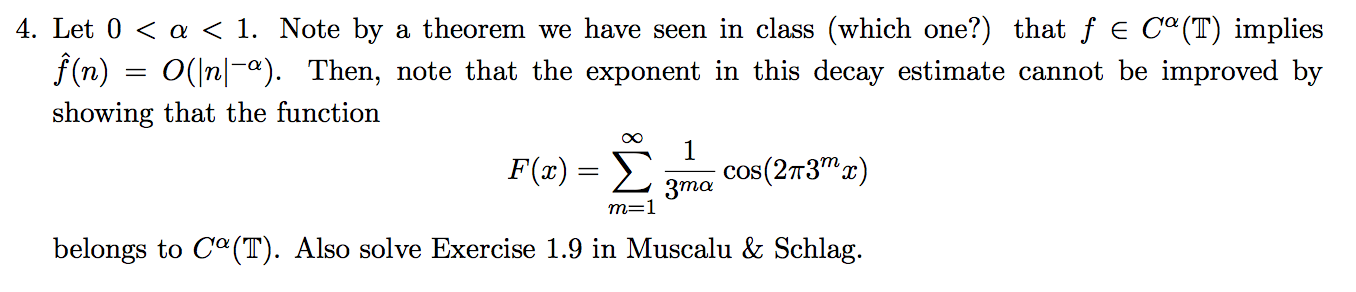
\includegraphics[width=1\textwidth]{HA-2-4.png}
\end{figure}
\end{question}
\begin{solution} \hfill \\
A theorem that gives this result of $f \in C^{\alpha}(\mathbb{T})
\implies \hat{f}(n) = O(n^{-\alpha})$ is recorded in section $1.4.4$, pg.18 of Schleg.

\bigskip
The following is the proof of the problem $1.9$ 
from Schleg. 
As we have $f,g \in L^2(\mathbb{T})$, by Corollary $1.6$, the given inequality is equivalent to
\eQb
\sum_{n \in \mathbb{Z}} |\widehat{f * g}(n)|^2 &\leq&
\sqrt{\sum_{n \in \mathbb{Z}} |\widehat{f * f}(n)|^2}  
\sqrt{\sum_{n \in \mathbb{Z}} |\widehat{g * g}(n)|^2}. \\
\eQe
Since $\widehat{f*g}(n) = \hat{f}(n)\hat{g}(n)$, the above inequality is again equivalent to
\eQb
\big( \sum_{n \in \mathbb{Z}} |\hat{f}(n)\hat{g}(n)|^2 \big)^2 &\leq&
\sum_{n \in \mathbb{Z}} |\hat{f}(n)|^4 
\sum_{n \in \mathbb{Z}} |\hat{g}(n)|^4. \\
\eQe
Expanding the LHS of the desired inequality yields
\eQb
\big( \sum_{n \in \mathbb{Z}} |\hat{f}(n)\hat{g}(n)|^2 \big)^2 &=&
\sum_{n \in \mathbb{Z}} |\hat{f}(n)\hat{g}(n)|^4 + 
\sum_{n > m} 2|\hat{f}(n)\hat{f}(m)\hat{g}(n)\hat{g}(n)|^2 \\
&\leq&
\sum_{n \in \mathbb{Z}} |\hat{f}(n)\hat{g}(n)|^4 + 
\sum_{n > m} |\hat{f}(n)\hat{g}(n)|^4 + |\hat{f}(m)\hat{g}(m)|^4 \\
&=& \sum_{n \in \mathbb{Z}} |\hat{f}(n)|^4 
\sum_{n \in \mathbb{Z}} |\hat{g}(n)|^4, \\
\eQe
where the last inequality
holds by the Cauchy-Schwarz inequality on the inner product space of $l^2(\mathbb{T})$.

 
\hfill $\qed$
\end{solution}

\bigskip

\begin{question}[5]
\hfill
\begin{figure}[h!]
  \centering
    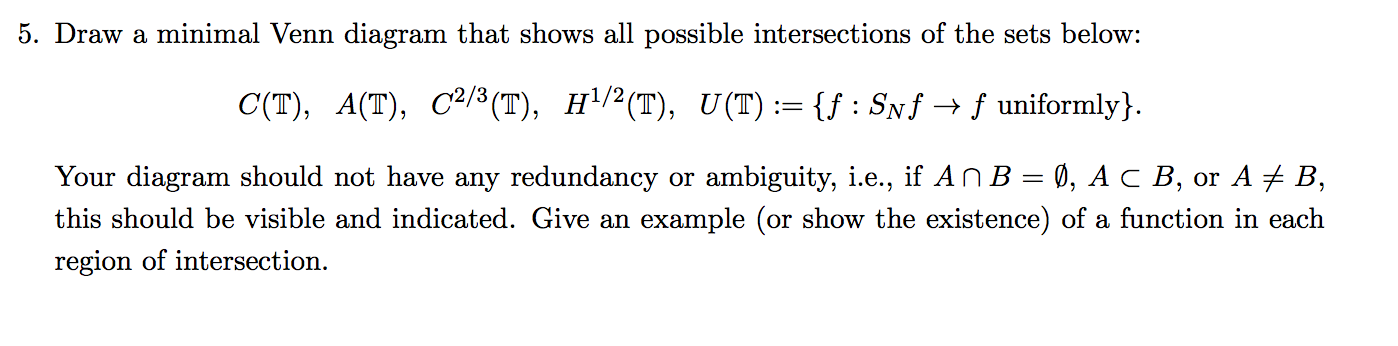
\includegraphics[width=1\textwidth]{HA-2-5.png}
\end{figure}
\end{question}
\begin{solution}
\hfill $\qed$
\end{solution}

\bigskip

\end{document}
